\documentclass[presentation,aspectratio=169]{beamer}
\usepackage[utf8]{inputenc}
\usepackage[T1]{fontenc}
\usepackage{graphicx}
\graphicspath{{./graphics/}}
\usepackage[main=ngerman,english]{babel}
\usepackage{tabularx,longtable,capt-of,fvextra,csquotes}
\MakeOuterQuote{"}
\usepackage{wrapfig,rotating}
\usepackage[normalem]{ulem}
\usepackage{amsmath,amssymb}
\usepackage{acro}
\usepackage[nonumberlist]{glossaries}
\makeglossaries
\renewcommand{\glossarysection}[2][]{}
\usepackage{hyperref}
\usepackage{listings,minted}
\usepackage[duration=20]{pdfpc}
\usetheme{metropolis}
\author{Julius Freudenberger}
\date{Cyberweek Sommersemester 2025}
\title{WYSIWYAF with \LaTeX}
\subtitle{Wissenschaftliche Arbeiten oder Präsentationen mit \LaTeX -- Fortgeschrittene}
\mode<presentation>{\usetheme{metropolis}}
\mode<beamer|handout>{\metroset{sectionpage=progressbar}}
\mode<beamer|handout>{\metroset{subsectionpage=progressbar}}
\mode<beamer|handout>{\metroset{progressbar=frametitle}}
\mode<beamer|handout>{\metroset{block=fill}}
\institute[Hochschule Esslingen]{Hochschule Esslingen}
\hypersetup{
  pdfauthor={Julius Freudenberger},
  pdftitle={WYSIWYAF with LaTeX -- Aufbaukurs},
  pdfkeywords={},
  pdfsubject={},
  pdflang={German},
  colorlinks,
  linkcolor=black,
  citecolor=black,
  filecolor=black,
  urlcolor=blue
}

\acsetup{locale/display,locale/format=\emph}
\DeclareAcronym{zB}{short=z.\,B.,long=zum Beispiel}
\DeclareAcronym{api}{short=API,
  long=Programmierschnittstelle,
  foreign=Application Programming Interface,
  foreign-locale=englisch,
  foreign-babel=english}
\DeclareAcronym{sw}{short=SW,long=Sammelwerk,long-plural=e}
\DeclareAcronym{ufo}{short=UFO,
  long=unidentifiziertes Flugobjekt,
  long-plural-form=unidentifizierten Flugobjekt,
  short-plural=}

\newglossaryentry{latex}
{
    name=\LaTeX,
    description={Markupsprache, die besonders für
      wissenschaftliche Dokumente und
      Präsentationen geeignet ist}
}



\usepackage{biblatex}

\begin{document}

\maketitle

\begin{frame}[fragile]{Bevor wir beginnen: Was brauche ich?}
  \begin{itemize}
    \item \LaTeX-Distribution: \TeX{}Live oder Mik\TeX{}
      \begin{itemize}
        \item Windows: \href{https://miktex.org/}{https://miktex.org/}
        \item Mac: \href{https://tug.org/mactex/}{https://tug.org/mactex/}
        \item Linux: Installation über den Paketmanager
          \begin{itemize}
            \item deb: \verb|texlive-base|, rpm: \verb|texlive texlive-latex|
            \item Arch Linux: \verb|texlive-core|
            \item NixOS: \verb|nixpkgs.texliveBasic|
          \end{itemize}
        \item Docker: \verb|texlive/texlive|
      \end{itemize}
    \item Texteditor
      \begin{itemize}
        \item \href{https://code.visualstudio.com/}{VSCode} mit \href{https://marketplace.visualstudio.com/items?itemName=James-Yu.latex-workshop}{\LaTeX-Workshop}, \href{https://www.vim.org/}{vim} mit \href{https://github.com/lervag/vimtex}{vimtex}
        \item \href{https://www.xm1math.net/texmaker/index.html}{\TeX{}Maker}
      \end{itemize}
    \item Alternativ: Online-Editoren
      \begin{itemize}
        \item Overleaf (\href{https://www.overleaf.com}{https://www.overleaf.com}, Registrierung erforderlich)
        \item \TeX{}Viewer (\href{https://texviewer.herokuapp.com}{https://texviewer.herokuapp.com}, direkt nutzbar)
      \end{itemize}
  \end{itemize}
\end{frame}

\begin{frame}{Über mich}
  \textbf{B.\,Eng. Julius Freudenberger}
  \begin{itemize}
    \item 2000 geboren
    \item 2016 erste Kontakte mit \LaTeX
    \item 2019 -- 2023 Bachelorstudium an der Hochschule Esslingen
    \item 2023 -- 2026(?) Masterstudium an der Hochschule Karlsruhe
    \item nebenbei Werkstudent
  \end{itemize}
\end{frame}

\begin{frame}{Wer seid ihr?}
  \begin{itemize}
    \item Name
    \item Fakultät? Was macht ihr da?
    \item Schon von \LaTeX{} gehört oder etwas damit gemacht?
    \item Was stört dich am meisten an traditionellen Textverarbeitungsprogrammen?
    \item Nächste (wissenschaftliche) Arbeit, die du vielleicht mit \LaTeX{} schreiben möchtest?
  \end{itemize}
\end{frame}

\begin{frame}{Materialien für den Kurs}
  \begin{itemize}
    \item Dieser Foliensatz
    \item Kleine Vorlagen zum Mitmachen
    \item Dokumente, die wir im Laufe des Kurses erstellen
      \bigskip
    \item wird alles im geteilten Ordner hochgeladen
  \end{itemize}
\end{frame}

\begin{frame}{Inhalt}
  \tableofcontents
\end{frame}

\section{Tabellen}

\begin{frame}{Setzen von Tabellen}
  \begin{itemize}
    \item Tabellen haben eigene Syntax in \LaTeX
    \item Ausrichtung einzelner Spalten kann individuell festgelegt werden
    \item Linien können für jede Spalte/Zeile individuell festgelegt werden
  \end{itemize}
\end{frame}

\begin{frame}[fragile]{Beispieltabelle}
  \begin{columns}
    \begin{column}{.49\textwidth}
      \begin{tabular}{|l|c|r|}
  \hline
  Hallo & Beispiel & Ende \\
  \hline
  Dies  & ist      & Zeile 2 \\
  \hline
\end{tabular}

    \end{column}
    \begin{column}{.5\textwidth}
      \inputminted{latex}{codebeispiele/table-simple.tex}
    \end{column}
  \end{columns}
\end{frame}

\begin{frame}[fragile]{Setzen von Tabellen}
  \begin{itemize}
    \item Spaltentrennung
      \begin{itemize}
        \item Spalten werden in jeder Zeile durch \verb|&| getrennt
        \item muss nicht zwingend untereinander stehen, sieht aber aufgeräumt im Code aus $\rightarrow$ hat keine Auswirkung auf die Formatierung der Tabelle
      \end{itemize}
    \item Zeilentrennung
      \begin{itemize}
        \item jede Zeile endet \emph{zwingend} mit \verb|\\|
        \item Linie wird mit \verb|\hline| erstellt
        \item muss zwischen allen Zeilen gesetzt werden, wo eine Linie auftauchen soll
      \end{itemize}
    \item Zweiter Parameter
      \begin{itemize}
        \item gibt an, wie viele Spalten es gibt und wie sie ausgerichtet sind
          \begin{itemize}
            \item \verb|c| -- centered
            \item \verb|l| -- left
            \item \verb|r| -- right
          \end{itemize}
        \item \verb/|/ gibt an, ob die Spalten durch eine Linie getrennt werden sollen
      \end{itemize}
  \end{itemize}
\end{frame}

\begin{frame}[fragile]{Beschriftung einer Tabelle}
  \begin{columns}
    \begin{column}{.45\textwidth}
      \begin{table}
  \begin{tabular}{c|c|c}
    Hallo & Beispiel & Ende \\
    \hline
    Dies  & ist      & Zeile 2 \\
  \end{tabular}
  \caption{Beispieltabelle mit
            Beschriftung}
\end{table}

    \end{column}
    \begin{column}{.5\textwidth}
      \inputminted{latex}{codebeispiele/table-float.tex}
    \end{column}
  \end{columns}
  \vspace{1em}
  \begin{itemize}
    \centering
    \item gleiche Platzierungsregeln wie bei anderen Floats gelten
  \end{itemize}
\end{frame}


\begin{frame}[fragile]{Einschränkungen von tabular}
  \begin{itemize}
    \item Wenn der Text zu lang ist, wird kein Zeilenumbruch gesetzt
      \begin{itemize}
        \item Abhilfe: Spalte mit \verb|p{...cm}| deklarieren oder
        \item \verb|\usepackage{tabularx}|
      \end{itemize}
    \item Tabellen mit \verb|tabular| können keine Seitenumbrüche
      \begin{itemize}
        \item Lange Tabellen werden am Ende der Seite einfach abgeschnitten
        \item Lösung: \verb|longtable|
      \end{itemize}
  \end{itemize}
\end{frame}

\begin{frame}[fragile]{tabularx}
  \begin{columns}
    \begin{column}{.35\textwidth}
      \begin{tabularx}{\textwidth}{X|X|X}
  % X sorgt für Umbruch
  % und "stretcht" die Spalte
  Hallo & Beispieltext & Ende \\
  \hline
  Dies  & ist      & Zeile 2 \\
\end{tabularx}

    \end{column}
    \begin{column}{.55\textwidth}
      \inputminted{latex}{codebeispiele/table-tabularx.tex}
    \end{column}
  \end{columns}
\end{frame}

\begin{frame}[fragile]{longtable}
  \inputminted{latex}{codebeispiele/table-longtable.tex}
\end{frame}

\begin{frame}{Beispiel für longtable}
  \begin{longtable}{c|c}
  Wird \emph{nur} auf der & ersten Seite oben gezeigt \\
  \endfirsthead
  Wird auf \emph{jeder}   & Seite oben gezeigt \\
  % Funktioniert nur leider in Präsentationen nicht
  \endhead
  Wird auf \emph{jeder}   & Seite unten gezeigt \\
  \endfoot
  Wird \emph{nur} auf der & letzten Seite unten gezeigt \\
  \endlastfoot
  Normaler                & Inhalt \\
  der                     & Tabelle \\
\end{longtable}

\end{frame}

\section{Weitere Verzeichnisse}

\begin{frame}[fragile]{Weitere Verzeichnisse}
  \begin{itemize}
    \item automatisch aktualisierendes Inhaltsverzeichnis sowie Verzeichnisse für Abbildungen, Codelistings (Abkürzungen, Stichwörter, Bibliographie, \dots)
  \end{itemize}
  \inputminted{latex}{codebeispiele/list-of-everything.tex}
\end{frame}

\subsection{Abkürzungen}

\begin{frame}{Abkürzungen mit acro}
  \begin{itemize}
    \item Liste von Abkürzungen mit ihrer langen Form
    \item automatisches Einfügen der richtigen Form
      \begin{itemize}
        \item lange Form beim ersten Auftreten
        \item Abkürzung sonst
        \item manuell überschreibbar
      \end{itemize}
    \item Pluralformen in Abkürzung und langer Form
    \item automatisches Verzeichnis der verwendeten Abkürzungen
  \end{itemize}
\end{frame}

\begin{frame}[fragile]{Einrichtung des Pakets}
  \inputminted{latex}{codebeispiele/acro-setup.tex}
\end{frame}

\begin{frame}[fragile]{Benutzte Abkürzungen in den Beispielen}
  \inputminted{latex}{codebeispiele/acro-used-acronyms.tex}
\end{frame}

\begin{frame}[fragile]{Setzen von Abkürzungen}
  \begin{columns}
    \begin{column}{.49\textwidth}
      \ac{zB}
\\% automatisch (1. Mal voll,
%               danach Abk.)
\ac{zB}\\
\acs{zB}
\\% Abkürzung
\acl{zB}
\\% lange Form
\acf{zB}
% volle Form (lange Form
% und Abkürzung in Klammern)

    \end{column}
    \begin{column}{.5\textwidth}
      \inputminted{latex}{codebeispiele/acro-usage.tex}
    \end{column}
  \end{columns}
\end{frame}

\begin{frame}[fragile]{Setzen von Abkürzungen}
  \begin{itemize}
    \item in den meisten Fällen reicht \verb|\ac|
    \item für Großschreibung (wie an Satzanfängen) ein großes \verb|A| in den Befehlen verwenden: \verb|\Ac|
  \end{itemize}
\end{frame}

\begin{frame}[fragile]{Besonderheiten in deutschen Texten -- Pluralformen}
  \begin{itemize}
    \item Pluralform nicht mit 's' gebildet
  \end{itemize}
  \inputminted[firstline=8,lastline=8]{latex}{codebeispiele/acro-used-acronyms.tex}
  \vspace{2em}
  \begin{columns}
    \begin{column}{.49\textwidth}
      \aclp{sw}

    \end{column}
    \begin{column}{.5\textwidth}
      \inputminted{latex}{codebeispiele/acro-german-plurals.tex}
    \end{column}
  \end{columns}
\end{frame}

\begin{frame}[fragile]{Besonderheiten in deutschen Texten -- Übersetzungen}
  geläufige englische Abkürzung für deutschen Begriff
  \inputminted[firstline=3,lastline=7]{latex}{codebeispiele/acro-used-acronyms.tex}
  \acf{api}

\end{frame}

\begin{frame}[fragile]{Besonderheiten in deutschen Texten -- Abweichender Kasus in langer Form}
  \begin{itemize}
    \item Bei langer Form bei der ersten Erwähnung wird das Wort in einem anderen Kasus benötigt
    \item Trick: Pluralform missbrauchen
  \end{itemize}
  \inputminted[firstline=9,lastline=12]{latex}{codebeispiele/acro-used-acronyms.tex}
  \vspace{2em}
  \begin{columns}
    \begin{column}{.49\textwidth}
      Wir widmen uns dem \acfp{ufo}.

    \end{column}
    \begin{column}{.5\textwidth}
      \inputminted{latex}{codebeispiele/acro-german-different-case.tex}
    \end{column}
  \end{columns}
\end{frame}

\subsection{Glossar}

\begin{frame}{Glossar mit glossaries}
  \begin{itemize}
    \item Liste von Wörtern mit ihren Erklärungen
    \item im Text wird Wort (mit Link auf das Glossar) gesetzt
    \item Glossar enthält alle benutzten Wörter und ihre Erklärungen
  \end{itemize}
\end{frame}

\begin{frame}[fragile]{Einrichtung des Pakets}
  \inputminted{latex}{codebeispiele/glossaries-setup.tex}
\end{frame}

\begin{frame}[fragile]{Setzen eines Wortes aus dem Glossar}
  \begin{columns}
    \begin{column}{.49\textwidth}
      Dieses Dokument wurde in
\gls{latex} gesetzt.

    \end{column}
    \begin{column}{.5\textwidth}
      \inputminted{latex}{codebeispiele/glossaries-usage.tex}
    \end{column}
  \end{columns}
\end{frame}

\begin{frame}{Resultierendes Glossar}
  %\minted{latex}{\printglossary}
  \printglossary
\end{frame}

\begin{frame}[fragile]{Besonderheit beim Kompilieren}
  \begin{itemize}
    \item Erstellung des Glossars geschieht mittels externem Befehl (ähnlich wie bei Literaturverzeichnissen)
    \item \verb|> makeglossaries <filename>|
    \vspace{1em}
    \item alternativ: anstatt \verb|\makeglossaries| \verb|\makenoidxglossaries| nutzen
    \item dann wird Sortierung intern gemacht (langsamer)
    \item zum Anzeigen des Glossars dann \verb|\printnoidxglossaries|
  \end{itemize}
\end{frame}

\section{Die Dokumentenklasse scrbook}

\begin{frame}[fragile]{Bücher?}
  \begin{itemize}
    \item nicht nur geeignet für Bücher
    \item kann auch für Abschlussarbeiten verwendet werden, besonders wenn diese gedruckt werden
    \item weist bestimmte Besonderheiten im Gegensatz zu z.\,B. \verb|scrartcl| auf
  \end{itemize}
\end{frame}

\begin{frame}[fragile]{Besonderheiten der Klasse scrbook}
  \begin{itemize}
    \item neue Überschriftsebene \verb|chapter|
    \item zweiseitiges Layout
      \begin{itemize}
        \item Seitenzahlen immer außen
        \item Kapitel beginnen immer auf einer rechten Seite
      \end{itemize}
    \item Gliederung in Abschnitte \verb|\frontmatter| \verb|\mainmatter| \verb|\backmatter|
      \begin{itemize}
        \item \verb|\frontmatter| römische Seitenzahlen
        \item \verb|\mainmatter| und \verb|\backmatter| arabische Seitenzahlen
      \end{itemize}
  \end{itemize}
\end{frame}

\section{Präsentationen}

\begin{frame}[fragile]{Präsentationen}
  \begin{itemize}
    \item Dokumentenklasse \verb|beamer|
    \item Präsentation besteht aus einer Abfolge von Folien
      \inputminted{latex}{codebeispiele/beamer-frame.tex}
  \end{itemize}
\end{frame}

\begin{frame}[fragile]{Präsentationen -- Besonderheiten}
  \begin{itemize}
    \item \verb|\section| oder \verb|\subsection| erstellen einzelne Folien mit den Überschriften
    \item \verb|\maketitle| erstellt Titelfolie
    \item zu langer Inhalt verschiebt sich nicht automatisch auf die nächste Folie
    \item Für Listings oder \verb|verbatim| muss der Frame als \verb|fragile| gekennzeichnet werden
      \inputminted{latex}{codebeispiele/frame-fragile.tex}
  \end{itemize}
\end{frame}

\begin{frame}[fragile]{"Animationen" -- Overlays}
  \begin{itemize}
    \item PDF kann keine bewegten Animationen
    \item aber Aufzählungspunkte oder anderer Inhalt kann nacheinander eingeblendet werden
    \item jedes Overlay wird auf einer neuen PDF-Seite angezeigt
      \inputminted{latex}{codebeispiele/beamer-overlays.tex}
  \end{itemize}
\end{frame}

\begin{frame}[fragile]{Themes}
  \begin{itemize}
    \item Klassische Themes in der \href{https://hartwork.org/beamer-theme-matrix/}{Beamer Theme Matrix}
    \item Modernes Theme (auch in dieser Präsentation): \href{https://ctan.org/pkg/beamertheme-metropolis}{Metropolis}
      \begin{itemize}
        \item Moderne Font (wenn mit Xe\LaTeX{} oder Lua\LaTeX{} kompiliert wird)
        \item kann optional einen Fortschrittsbalken anzeigen
        \item Einstellungen mit \verb|\metroset|
      \end{itemize}
  \end{itemize}
\end{frame}

\begin{frame}[fragile]{Bewerbungsunterlagen}
  \begin{columns}
    \column{.5\textwidth}
      \centering
      \begin{itemize}
        \item Lebenslauf mit \verb|moderncv|
      \end{itemize}
      
\includegraphics[height=.7\textheight]{Lebenslauf}
    \column{.5\textwidth}
      \centering
      \begin{itemize}
        \item Anschreiben mit \verb|dinbrief|
      \end{itemize}
      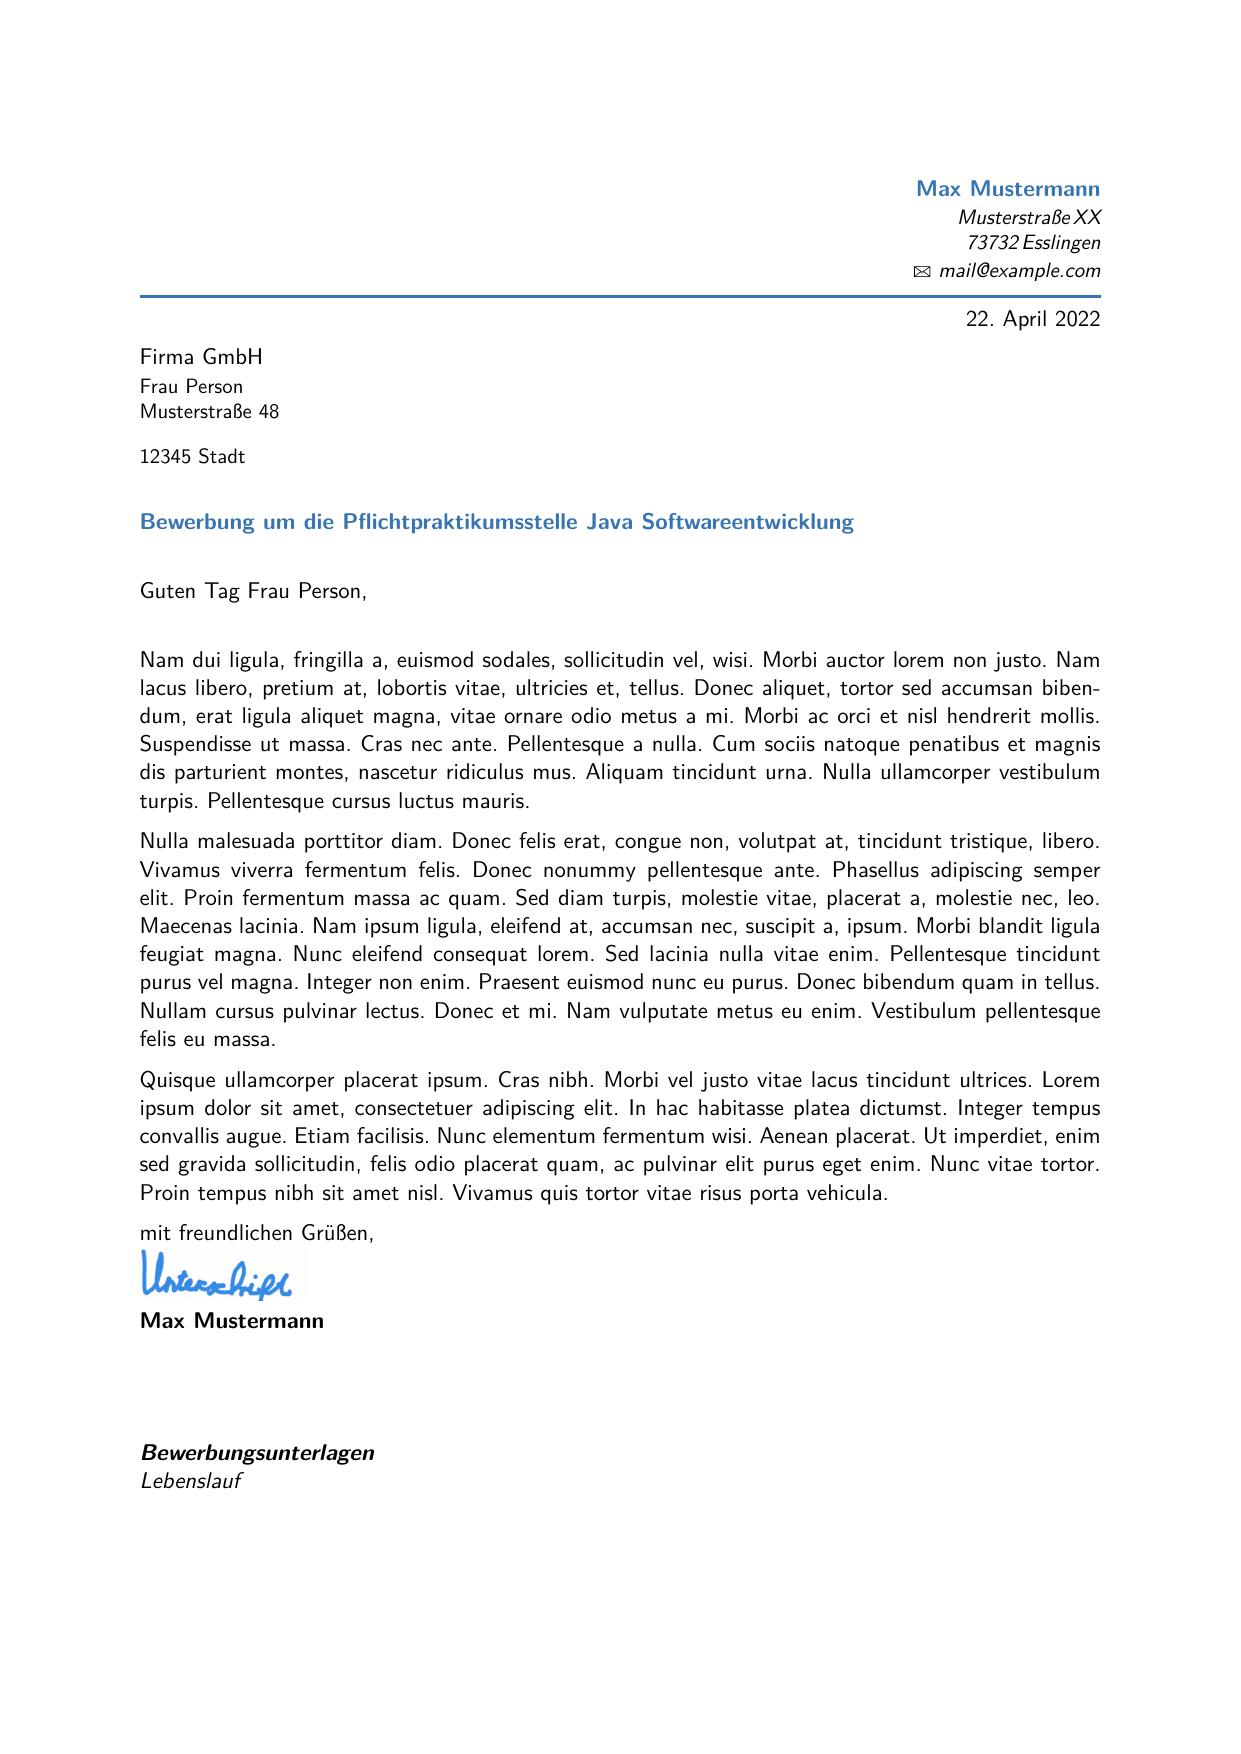
\includegraphics[height=.7\textheight]{Anschreiben}
  \end{columns}
\end{frame}

\begin{frame}[fragile]{Wohin bei Problemen?}
  \begin{itemize}
    \item \verb|texdoc <paketname>|
    \item Suchmaschine des Vertrauens
    \item \href{https://de.wikibooks.org/wiki/LaTeX-Kompendium}{\LaTeX-Kompendium}
    \item \href{https://www.overleaf.com/learn}{Overleaf documentation}
    \item \href{https://golatex.de/wiki/index.php/Hauptseite}{Go\LaTeX-Wiki}
    \item \href{https://tex.stackexchange.com}{\TeX-Stackexchange}
  \end{itemize}
\end{frame}

\maketitle

\end{document}
